\documentclass[../main.tex]{subfiles}

\graphicspath{{../images/}}

\begin{document}
\hrule
\section{Bound States}
\hrule \vspace{10px}

\lhead{Lecture 10: 2/19/24}
\chead{Bound States}
\rhead{PHYS 474}

\paragraph*{Two Types:}
\begin{itemize}
    \item Binding Energy $<$ Rest mass energy: Nonrelativistic bound state e.g. Hydrogen atom
    (-13.6 eV $<$ 1GeV rest mass of proton). 
    \item Binding Energy $>$ Rest mass energy: Relativistic bound state e.g. light meson.
\end{itemize}
\paragraph*{Hydrogen Atom:} The potential energy is given by
\begin{align*}
    V(r) = -\frac{e^2}{r}
\end{align*}
or the coulomb potential. The Hamiltonian is given by the Schr\"odinger equation
\begin{align*}
    H\psi = -\frac{\hbar}{2m} \laplacian \psi(\vb r) + V(r) \psi(\vb r) = E\psi(\vb r)
\end{align*}
where $V(r)$ is the central potential with spherical symmetry SO(3). But there also is an enhanced 
symmetry.
\paragraph*{Noether's Theorem:} Symmetry $\leftrightarrow$ Conservation Law. e.g. 
\begin{itemize}
    \item SO(3) $\leftrightarrow$ Conservation of Angular momentum. 
    \item SO(1,3) $\leftrightarrow$ linear momentum (Poincare symmetry)
    \item T-reversal $\leftrightarrow$ energy
    \item U(1)$_{em}$ $\leftrightarrow$ electric charge
\end{itemize}
so from the central potential, we know that angular momentum $\vb L$ is conserved. But for
$1/r$ there is a SO(4) symmetry from the LRL (Laplace-Runge-Lenz) vector
\begin{align*}
    \mathcal{L} = \frac{1}{m} \vb L \cross \vb p + \frac{\kappa \vb r}{r}
\end{align*}
where
\begin{align*}
    V(r) = -\frac{\kappa}{r}
\end{align*}
the energy eigenvalues of the hydrogen atom are given by
\begin{align*}
    E_n = -\frac{\qty{13.6}{eV}}{n^2} = -\frac{m e^4}{2\hbar^2 n^2}
     = -\frac{1}{2} \frac{\alpha m_e c^2}{n^2}
\end{align*}
where $\alpha = \frac{e^2}{\hbar c} \approx \frac{1}{137}$ is the fine structure constant.
\paragraph*{Degeneracy} $n^2$ e.g.
% table of n l m and degeneracy
\begin{table}[ht]
    \centering
    \begin{tabular}{c|c|c|c}
        n & l & m & degeneracy \\
        \hline
        1 & 0 & 0 & 1 \\
        \hline
        2 & 0 & 0 & 1 \\
         & 1 & -1,0,1 & 3 \\
        \hline
        3 & 0 & 0 & 1 \\
        & 1 & -1,0,1 & 3 \\
        & 2 & -2,-1,0,1,2 & 5 \\
    \end{tabular}
\end{table}
For SO(3), $(2l + 1)$ degeneracy
\begin{align*}
    \sum_{l=0}^{n-1} (2l + 1) = 2\sum_{l=0}^{n-1} l + n = 2 \frac{(n - 1)(n)}{2} + n = n^2
\end{align*}
\paragraph*{Positronium} ($e^+ e^-$ bound state) has the same energy levels as the hydrogen atom
the energy eigen value is given by first looking at the reduced mass
\begin{align*}
    \mu = \frac{1}{\frac{1}{m_e} + \frac{1}{m_e}} = \frac{m_1m_2}{m_1 + m_2} \approx m_1    
    \qqtext{if} m_1 \ll m_2
\end{align*}
but here $m_1 = m_2 = m_e$ so $\mu = \frac{m_e}{2}$. The energy eigenvalues are given by
\begin{align*}
    E_n = \frac{1}{2} -\frac{\qty{13.6}{eV}}{n^2} = -\frac{\qty{6.8}{eV}}{n^2}
\end{align*}
We can do this for Muonium ($\mu^+ e^-$ bound state) and Pionic Hydrogen($\pi^+ e^-$ bound state).
\paragraph*{Fine Structure}
\begin{enumerate}
    \item Relativistic Correction
    \begin{align*}
        T = E - m_ec^2
    \end{align*}
    \item Spin-Orbit Coupling
    \item Lambd Shift (QED)
    \item Hyperfine Splitting aka zeeman effect
\end{enumerate}

\newpage
\lhead{Lecture 11: 2/21/24}

\paragraph*{Quiz Review} 
\begin{itemize}
    \item For the Positronium:
    \begin{align*}
        C: (-1)^{l+s} = (-1)^n
    \end{align*}
    where $l + s = n$ (the selection rule for Positronium decay). *for $n$ photons, $C = (-1)^n$. 
    FOr the ground states $l = 0$ so the spin is
    \begin{align*}
        S: \ohf \otimes \ohf = 1 \oplus 0
    \end{align*}
    where we have a triplet state $S = 1$ and a singlet state $S = 0$. For this singlet:
    \begin{align*}
        S = 0 \implies (-1)^0 = 1 = (-1)^2
    \end{align*}
    or two photons can be emitted (para-positronium). For the triplet state:
    \begin{align*}
        S = 1 \implies (-1)^1 = -1 = (-1)^3
    \end{align*}
    or three photons can be emitted (ortho-positronium). The mass of each photon for two photons is
    roughtly a half of the mass of the positronium $E_\gamma = \qty{511}{keV}$. For three photons
    $E_\gamma < 511$ keV. 
    \item Binding Energy vs. Rest Mass Energy: Quarkonium ($q \bar q$): $uds$ light quarks,
    $cbt$ heavy quarks.
    \begin{itemize}
        \item Heavy Quarkonium: $c\bar c$: Charmonium ($J/\psi$), $b\bar b$: Bottomonium
        ($\Upsilon$), $t\bar t$: Toponium \emph{does not exist}
        (very heavy so it decays really fast $\sim 10^{-25}$s vs
        $\tau_{\text{bound state}} \sim 10^{-23}$ sec).
    \end{itemize}
    For Charmoniun, the reduced mass is 
    \begin{align*}
        \mu = \frac{m_c m_c}{m_c + m_c} \approx \frac{m_c}{2}
    \end{align*}
    and the energy of the Hydrogen atom is
    \begin{align*}
        E_n = -\frac{m e^4}{2\hbar^2 n^2} = -\frac{1}{2} \frac{\alpha m c^2}{n^2}
    \end{align*}
    and for the Charmonium:
    \begin{align*}
        E_n = -\frac{4}{9} \frac{1}{2} \frac{\alpha m_c c^2}{n^2} \qqtext{incorrect}
    \end{align*}
    where we have to adjust for the charge of the quark $e \to \frac{2}{3}e$ and the potential:
    For electron coulomb potential we know that 
    \begin{align*}
        V = -\frac{e^2}{r} = -\frac{e^2}{\hbar r}\frac{\hbar c}{r} = -\frac{\alpha \hbar c}{r}
    \end{align*}
    but for quarks there is a different potential from the strong interaction (gluon)
    \begin{align*}
        V(r) = -\frac{\alpha_s \hbar c}{r} - \frac{4}{9} \frac{\alpha \hbar c}{r}
        \qquad \alpha_s = \frac{g_s^2}{\hbar c} \gg \alpha
    \end{align*}
    which is much larger than the coulomb potential (suppressed second term), but there is a
    transition to a linear potential as the distance get very large.
    \begin{align*}
        V(r) = -\frac{4}{3} \frac{\alpha_s \hbar c}{r} + F_o r \qqtext{QCD Potential}
    \end{align*}
    there also is a color factor $\frac{4}{3}$ based on the three colors of the quarks.
    So the energy is given by
    \begin{align*}
        E_n = -\frac{4}{3} \frac{1}{2} \frac{\alpha_s m_c c^2}{n^2}
    \end{align*}
    \item Decay of Charmonium:
    \begin{align*}
        J/\psi \to \pi^+ \pi^- \pi^0 \qor D^+ D^-
    \end{align*}
    For the ground state, $m_{J/\psi} = 3.1$ GeV. And the total rest mass of $D^+ D^-$ is 
    kinematically forbidden $m_{D^+} + m_{D^-} = 3.7$ GeV. We have a decay to 3 pions due to
    the G-parity conservation $(-1)^I C$ or $(-1)^{n}$.

    \paragraph*{OZI rule} (Okubo, Zweig, Iizuka) Cutting a hard gluon line in the Feynman diagram
    separates the quarks and the decay is suppressed. For soft gluon lines, cutting a line does not
    separate the quarks and the decay is not suppressed.
    \begin{figure}[ht]
        \centering
        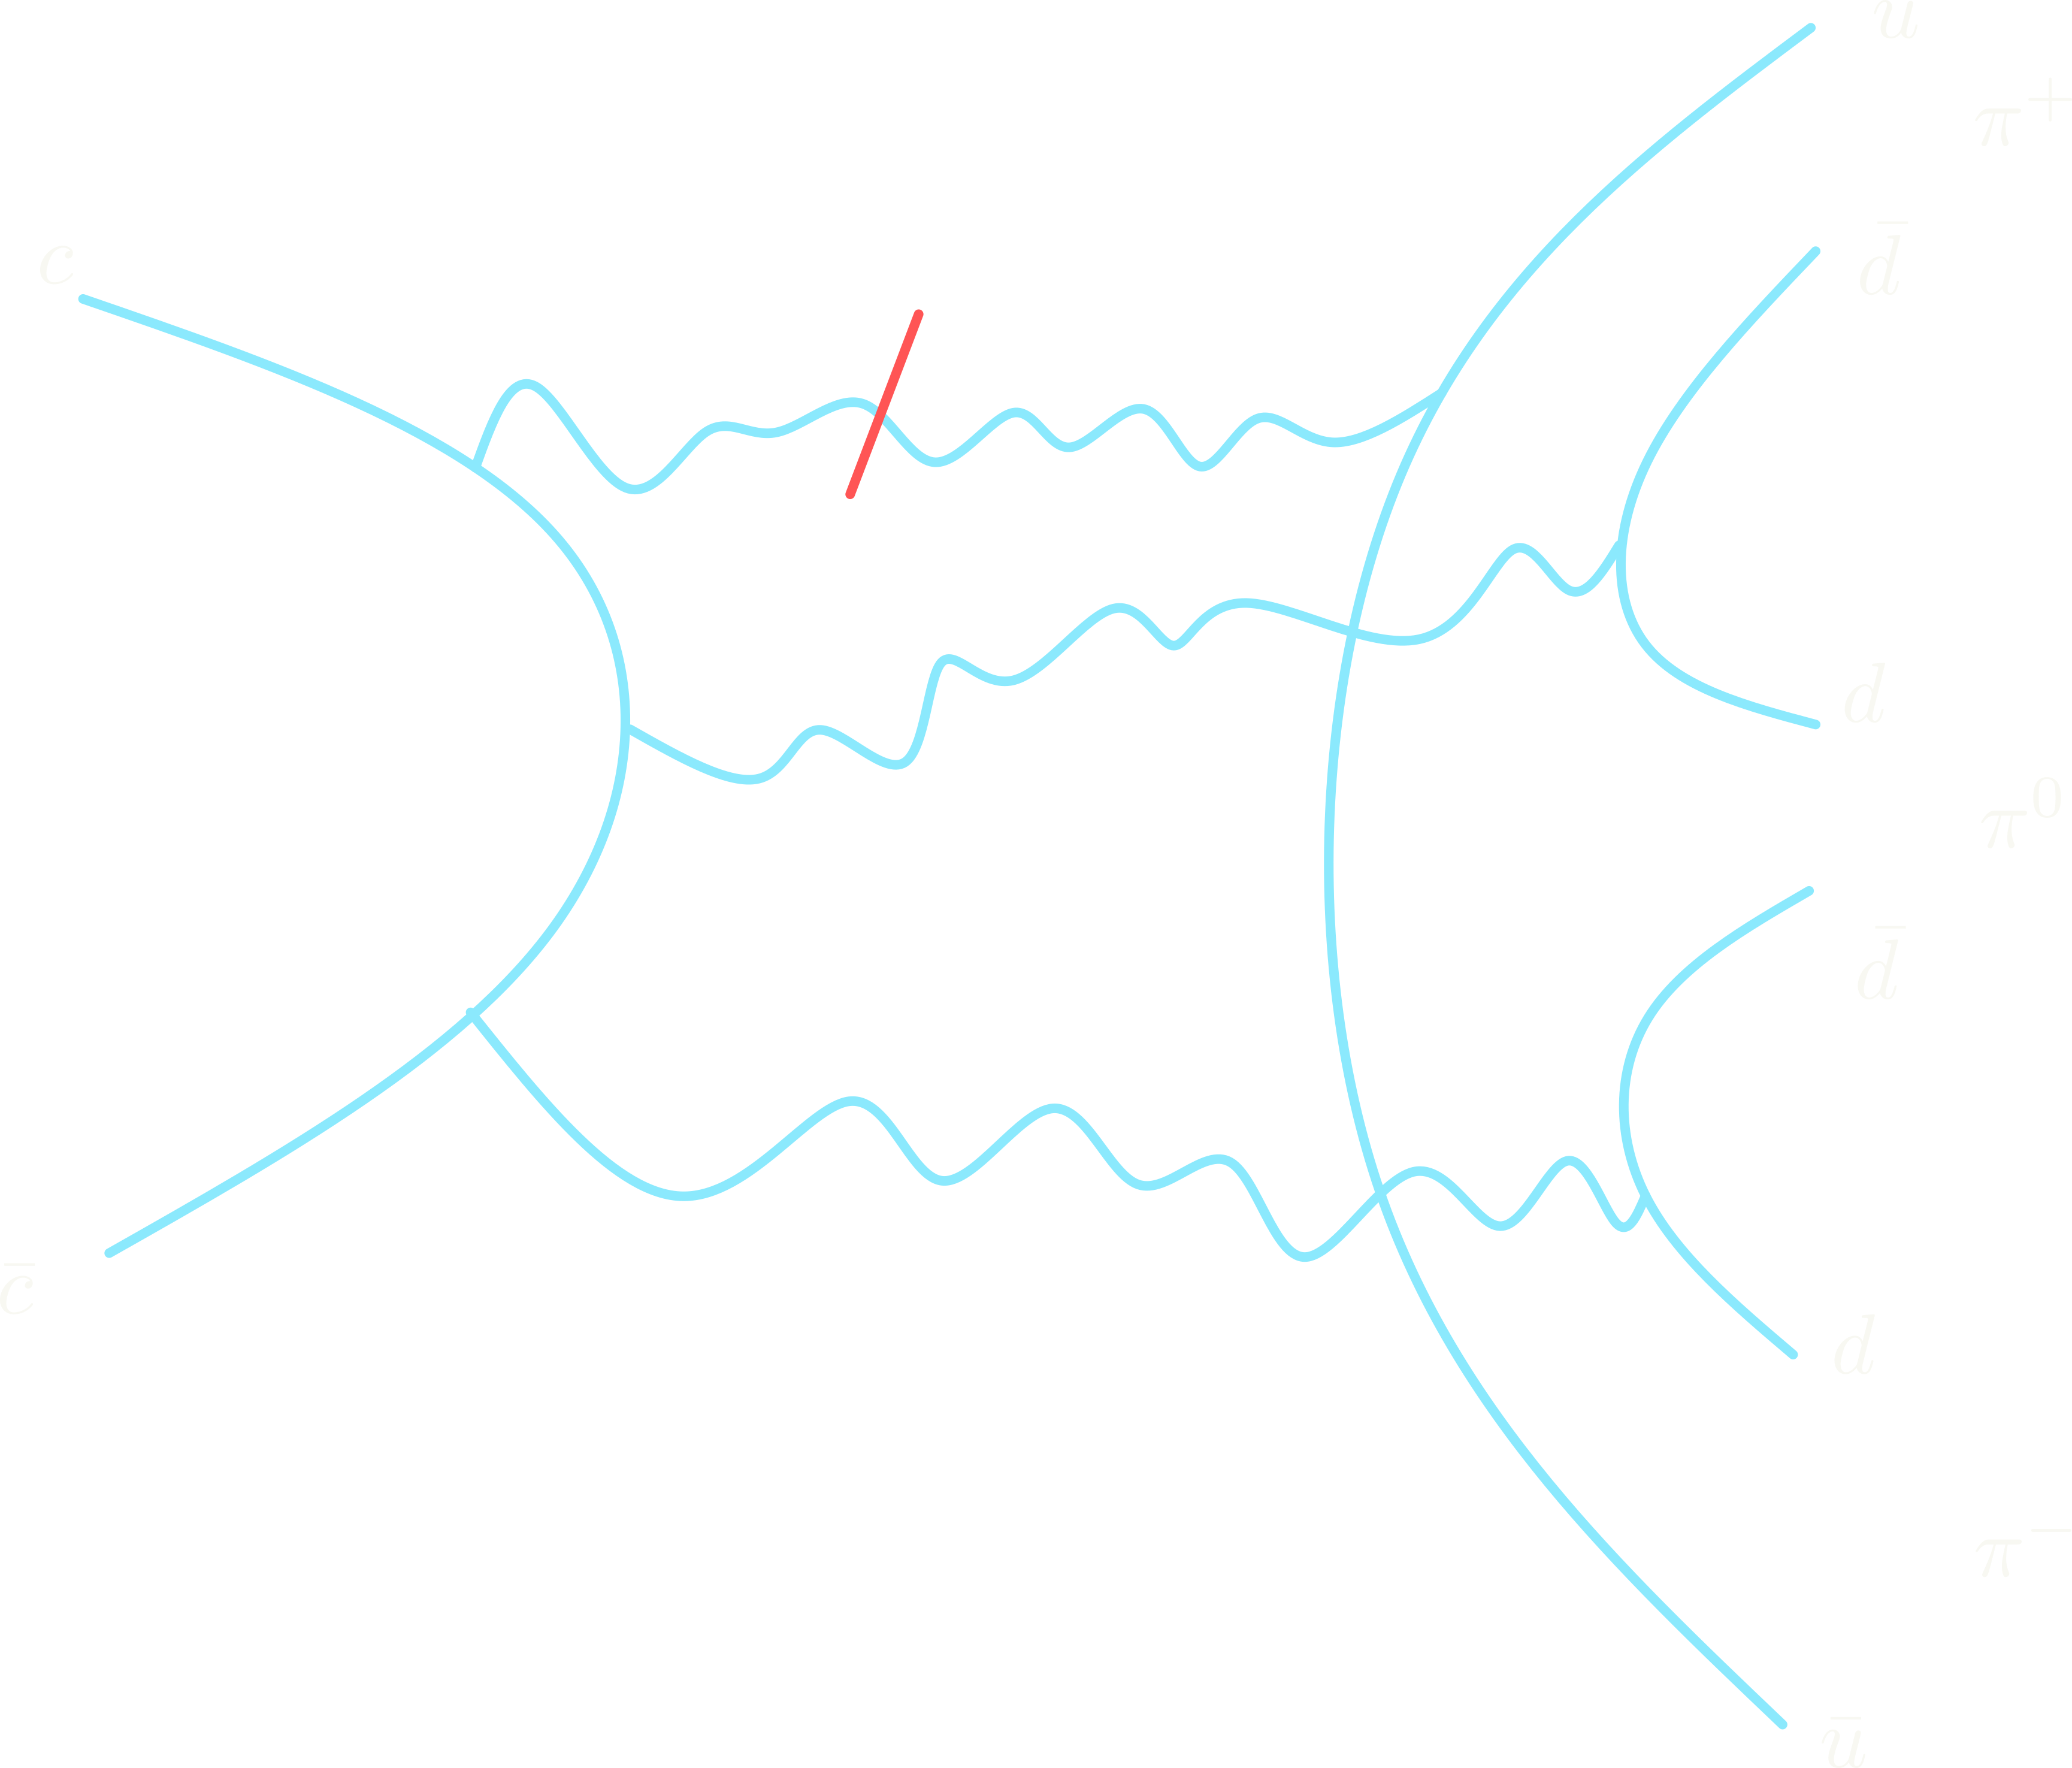
\includegraphics[width=0.5\textwidth]{ozirule.png}
        \caption{OZI Rule}
        \label{fig:ozi}
    \end{figure}
    \item Light Mesons: $q\bar q$ where $q = u,d,s$. There are nine spin-0 (pseudo scalar) mesons
    and nine spin-1 (vector) mesons. (insert figure 5.11 from Griffiths). From the lie algebra
    of the spin-0 nonet
    \begin{align*}
        3 \otimes \bar 3 = 8 \oplus 1
    \end{align*}
    where the 1 is the $\eta'$ meson. and we break down the 8 into
    \begin{align*}
        8 \to 2 \oplus 3 \oplus 2 \oplus 1
    \end{align*}
    where they refer to the top row, middle row pions, bottom row and $\eta$ meson. For the vector
    mesons. For the isospin doublet:
    \begin{align*}
        u = \ket{\ohf \ohf} \qquad d = \ket{\ohf -\ohf}
    \end{align*}
    and for the antiquarks:
    \begin{align*}
        \bar u = \ket{\ohf -\ohf} \qquad \bar d = -\ket{\ohf \ohf}
    \end{align*}
    and the pions are given by
    \begin{align*}
        \pi^+ &= \ket{\ohf \ohf} \otimes \ket{\ohf \ohf} = - u \bar d \\
        \pi^- &= \ket{\ohf -\ohf} \otimes \ket{\ohf -\ohf} = d \bar u \\
        \pi^0 &= \frac{1}{\sqrt{2}}
            \qt(\ket{\ohf -\ohf} \otimes \ket{\ohf \ohf} + \ket{\ohf \ohf} \otimes \ket{\ohf -\ohf})  \\
        &= \frac{1}{\sqrt{2}} (u \bar u - d \bar d)
    \end{align*}
    for the corner mesons:
    \begin{align*}
        K^0 = d \bar s \qquad \bar K^0 = \bar d s \qquad K^+ = u \bar s \qquad K^- = \bar u s
    \end{align*}
    and the $\eta$ mesons are
    \begin{align*}
        \eta' &= \frac{1}{\sqrt{3}} (u \bar u + d \bar d + s \bar s) \\
        \eta &= \frac{1}{\sqrt{6}} (u \bar u + d \bar d - 2s \bar s)
    \end{align*}
    For spin-1 mesons, in terms of the flavor
    \begin{align*}
        \rho^+, \rho^0, \rho^- = \pi^+, \pi^0, \pi^- 
    \end{align*}
    and the same for the $K^*$ mesons. The difference is in the center
    \begin{align*}
        \omega = \frac{1}{\sqrt{2}} (u \bar u + d \bar d) \qquad \phi = s \bar s
    \end{align*}
\end{itemize}
\end{document}